\documentclass[10pt,a4paper,notitlepage]{article}
\setlength{\parskip}{3mm}
\setlength{\parindent}{0mm}
\usepackage[utf8]{inputenc}
\usepackage{amsmath}
\usepackage{amsfonts}
\usepackage{amssymb}
\usepackage{graphicx}
\usepackage[left=2cm,right=2cm,top=2cm,bottom=2cm]{geometry}
\usepackage{amsthm}
\usepackage{anyfontsize}
\title{Samasya}
\author{A p}
\date{7th August}
\begin{document}
%\maketitle

$$\mathrm{\textbf{\fontsize{30}{40}\selectfont Samasya}}$$

Samasya is a mathematics discussion and problem solving club. We discuss a variety of mathematical topics and solve problems as well. This week's meeting will be held at 9 p.m. on the $7^\mathrm{th}$ of August (Friday) in the UG MLH. We encourage participants to have a look at these problems\footnote{The problems are not necessarily in the order of difficulty} before the meeting. Discussion, however, will not be limited  to these problems. Participants can bring their own problems or mathematical ideas they wish to discuss.
\\
\hrule

\textbf{Problem 1.}
We have $2^m$ sheets of paper, with the number $1$ written on each of them. We perform the following operation. In every step we choose two distinct sheets; if the numbers on the two sheets are $a$ and $b$, then we erase these numbers and write the number $a + b$ on both sheets. Prove that after $m2^{m -1}$ steps, the sum of the numbers on all the sheets is at least $4^m$ .

\textbf{Problem 2.}
Consider the game rit. In this game you have a plus shaped board filled with marbles. It looks something like figure \ref{fig:fig1}.
The game progresses by `jumping' a marble over its adjacent marble on to an empty hole as shown in figure \ref{fig:fig2}. The marble that gets jumped over is removed from the board. The game goes on this way until no further moves can be made. You win the game if you end up with just one marble on the board. Show that if the game ends with just one marble, it can only end with the marble being in one of the holes marked in figure \ref{fig:fig3}.
\begin{figure}[h]
\centering
\fbox{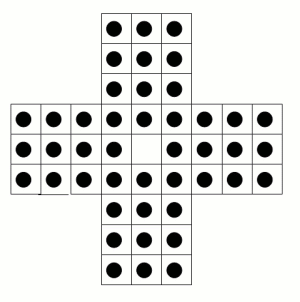
\includegraphics[scale=0.45]{board.png}}
\caption{The board of rit at the start of the game with all but the centre hole filled}
\label{fig:fig1}
\end{figure}

\begin{figure}[h]
\centering
\fbox{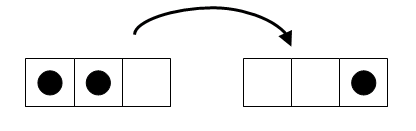
\includegraphics[scale=0.45]{move.png}}
\caption{A move of the game}
\label{fig:fig2}
\end{figure}

\begin{figure}[h]
\centering
\fbox{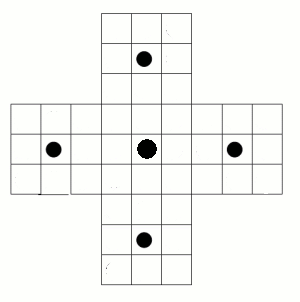
\includegraphics[scale=0.45]{board_end.png}}
\caption{All possible winning configurations?}
\label{fig:fig3}
\end{figure}

\textbf{Problem 3.}
Construct a tetromino by attaching two $2 \times 1$ dominoes along their longer sides such that the midpoint of the longer side of one domino is a corner of the other domino. This construction yields two kinds of tetrominoes with opposite orientations. Let us call them $S$- and $Z$-tetrominoes, respectively.
Assume that a lattice polygon $P$ can be tiled with $S$-tetrominoes. Prove that no matter how we tile $P$ using only $S$- and $Z$-tetrominoes, we always use an even number of $Z$-tetrominoes.

\textbf{Problem 4.}
Consider points $A, B, C, D$ in that order. Assume $CD > AB$ and $CB > AD$. Let $E$ be the point on $CD$ such that $ED = AB$ and let $F$ be the point on $BC$ such that $FB = AD$. Let the midpoint of $EF$ be $M$. Prove that $BM \perp MD$.

\textbf{Problem 5.}
A point $x$ on the real line is said to be a limit point of the set $A$ if for every $\delta >0$, $(x- \delta, x+\delta) \cap A \neq \emptyset$. 
\begin{itemize}

\item Show that for every uncountable subset $B$ of $\mathbb{R}$, at most countably many points of $B$ are \emph{not} limit points of $B$.

\item Prove that every monotonic function on an interval in $\mathbb{R}$ has at most countably many discontinuities.

\end{itemize}
\textbf{Problem 6.}
A set is \emph{closed} if it contains all its limit points. Find all sets $S \subset \mathbb{R}$ which are closed and also have the property that if $a,b \in S$, $a < b$, then there exists an $x \in S$ such that $a < x < b$.

\end{document}
